\documentclass[a4paper]{article}
\usepackage[english]{babel}
\usepackage{graphicx}
\usepackage{multicol}
\usepackage{amsmath}
\usepackage{hyperref}
\usepackage{amsthm}
\usepackage{geometry}
\geometry{a4paper} 
\usepackage{fancyhdr}
\usepackage{xcolor}
\usepackage{amssymb}
\usepackage{multicol}
\theoremstyle{definition}
\newtheorem{definition}{Defintion}[section]
\newtheorem{exmp}{Example}[section]
\newtheorem{theorem}{Theorem}

\begin{document}
\author{Fractals}
\title{\textbf{Functions}}
\maketitle
\tableofcontents
\noindent
\section{Introduction}
\subsection{Defintions}

\begin{definition}
    A function \(f\) from a set \(X\) to a set \(Y\) is a relation that assigns to each element in
    set \(X\) exactly one element in set \(Y\).
\end{definition}

\begin{definition}
    The domain is the set of \(X\) (a.k.a. the input).
\end{definition}

\begin{definition}
    The range is a subset of Y (a.k.a. the output).
\end{definition}

\subsection{Existence of a Function}
\begin{theorem}[\textbf{Vertical Line Test}]
    if you can draw a Vertical line that passes through more than one point of a
    relation on a grap, it's not a function, if you cannot, it's a function.

\end{theorem}


\begin{exmp}
    what the domain and range of the function \(f(x) = \sqrt{16 - x^2}\)?
\end{exmp}

\(sloution\) Note that if \(a < 0 \), then \( \sqrt{a}\) is undefined for reals,
Thus, \(16 - x^2 \ge 0 \Rrightarrow \) \framebox[\width]{
    \(-4 \le x \le 4\)
} since \(x^2 \ge 0\), we have that \(0 \le 16 - x^2 \le 16\),
so the range is \framebox[\width]{ \(0 \le y \le 4\) }


\section{Combinations of Functions}
\begin{theorem}[\textbf{common function Combinations}]
    The following are some common combinations of functions:
    \begin{itemize}
        \item \textbf{Sum} \((f+g)(x) = f(x) + g(x)\)
        \item \textbf{Differnce} \((f-g)(x) = f(x) - g(x)\)
        \item \textbf{Product} \((fg)(x) = f(x)g(x)\)
        \item \textbf{Quotient} \((\dfrac{f}{g} )(x) = \dfrac{f(x)}{g(x)} \)
              where \(g(x) \ne 0\)
        \item \textbf{Compostion} \((f\circ g)(x) = f(g(x))\)
    \end{itemize}

\end{theorem}

\begin{exmp}
    if \(f(x) = 2x + 3\) and \(\quad g(x) = 2x - 3\), then what is \(fg(4)\)?
\end{exmp}
\(sloution\) \( (fg)(x) = (2x+3)(2x-3) \) Thus \((fg)(4) = 55\).
\subsection{Domain and Range of a Composite Function}
The domain of a composite function is the intersection of domains of the starting
and final function.

\noindent
The range of a composite function is the range of the final function restricted by the
starting function.

\begin{exmp}
    let \(f(x) = \dfrac{1}{x+2}\) and \( \dfrac{x}{x-3} \).
    Then \(g(x)\) is the starting function and \( f(g(x)) \) is the final
    function. Find the domain and range of \(f(g(x))\).
\end{exmp}

\noindent
\(sloution\) \(f(g(x)) = \dfrac{1}{\dfrac{x}{x-3} + 2}\) so \(x \ne 3\),
impleing the domain is \framebox[\width]{ \(x \ne 2,3\) }.

\begin{exmp}
    If \(f(x) = \sqrt{x}\) and \(g(x) = x - 1\), what is the domain and range
    of \((g\circ f)(x)\)?
\end{exmp}
\noindent
\(sloution\) \((g\circ f)(x) = \sqrt{x} - 1\) it's obivious that \(x \ge 0\),
and all other values work, so the domain is \framebox[\width]{ \(0 \le x < \infty \ \)}
. Since \( \sqrt{x} \ge 0\)we have \((g\circ f)(x) \ge -1\), with no other restrictions,
so the range is \framebox[\width]{ \([-1,\infty] \) }.

\section{Types of Functions}
\subsection{Piecewise-Defined Function}
A piecewise function is a function that is defined by two or more equations over a
specified domain.

\begin{exmp}
    let \(f(x) = |x|\) Then
    \[ f(x) =
        \begin{cases}
            x  & \text{if } x \ge 0 \\
            -x & \text{if } x < 0
        \end{cases}
    \]

\end{exmp}

\begin{exmp}
    What are the domain and range of the piecewise function as follows?
    \[
        f(x) =
        \begin{cases}
            x^2 + 1 & x < 0   \\
            x - 1   & x \ge 0
        \end{cases}
    \]
\end{exmp}

\(sloution\). The domain includes \(x < 0 \) and \(x \ge 0\),
which is all values, so the domain is
\framebox[\width]{ \((-\infty, \infty)\) }. for \(x \ge 0\), we have \(f(x) = x - 1\),
so the range is \(y \ge -1\). For \(x < 0\) we have \(f(x) = x^2 + 1\), so the range is \(y > 1\).
Thus the range together is \framebox[\width]{ \([-1, \infty )\) }

\section{Properties of Functions}
\subsection{Odd and Even Functions}
A function \(f\) is even if \(f(x) = f(-x)\)


\begin{figure}[h]
    \begin{small}
        \begin{center}
            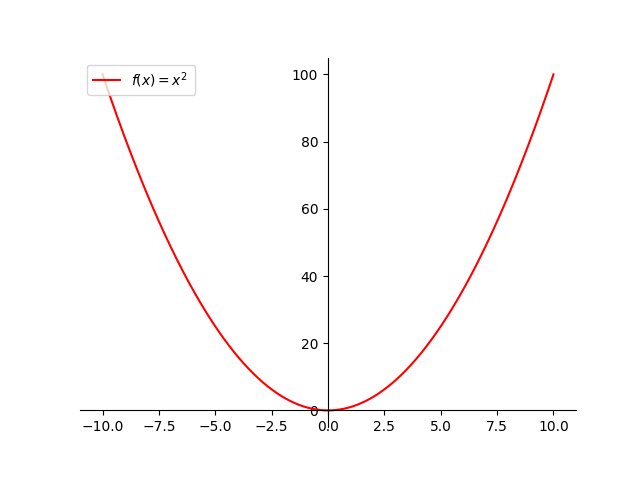
\includegraphics[width=0.75\textwidth]{../out/graphs.png}
        \end{center}
        \caption{Graph of an even function.}
        \label{fig: Even Function}
    \end{small}
\end{figure}

% \begin{center}
%     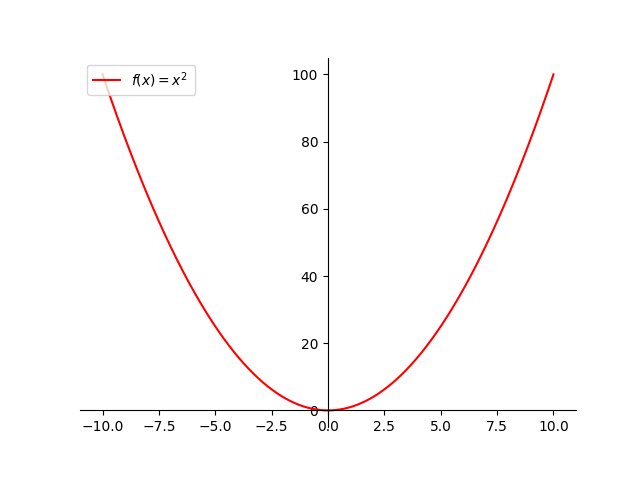
\includegraphics[width = 8cm]{../out/graphs.png}
% \end{center}
\subsection{Periodic Functions}
\section{Inverse Functions}
\subsection{Existence of an Inverse Function}
\end{document}
